\section{Depuração}
%%%%%%%%%%%%%%%%%%%%%%%%%%
\begin{frame}[fragile]
\frametitle{Depuração}
\begin{minipage}{0.47\textwidth}
    \begin{itemize}
        \item O que é depuração?
        \item Como funciona no Picat? 
        \item Exemplo de uso
    \end{itemize}
\end{minipage}
\begin{minipage}{0.5\textwidth}
\begin{figure}[ht!]
\begin{center}

\includegraphics[width=1.2\textwidth, height=0.40\textheight]{figures/logo_picat_alex.jpg}
\end{center}
\end{figure}
\end{minipage}
\end{frame}
%%%%%%%%%%%%%%%%%%%%%%%%%%
\begin{frame}[fragile]

    \frametitle{Depuração -- Quando usar?}

    \begin{itemize}
      \item Depuração,  \textit{trace} ou \textit{debug} -- o que é?
      \pause
      Mostrar estado de variáveis, funções e predicados durante a execução de um código
    
      \item Depuração ou \textit{trace} -- quando usar?
      \pause
     \textbf{\textcolor{violet}{Aprender detalhes da linguagem}}

  \pause
  \item Depuração ou \textit{trace} $\Rightarrow $      \textbf{\textcolor{violet}{para descobrir o erro!}}

\pause
    \item Em Picat não há um ambiente gráfico de depuração, 
    ao contrário do SWI-Prolog. 
      \pause
    Eis uma oportunidade de um projeto aqui....
        
    \item Contudo, o \textit{trace} do Picat faz tudo ...
      \pause
    
    \end{itemize}
\end{frame}

\begin{frame}[fragile]

\frametitle{Depuração -- Como funciona um predicado?}

\begin{figure}[!htb]
\begin{center}
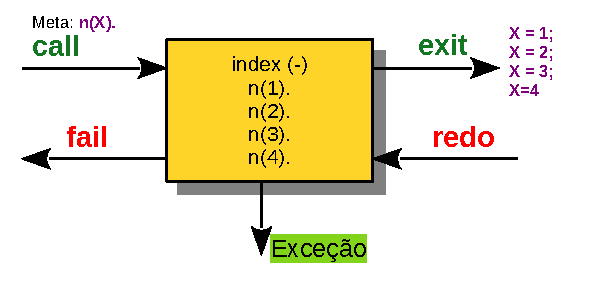
\includegraphics[width=0.90\textwidth, height=0.5\textheight]{figures/trace01.pdf}
%\caption{Realizar buscas com regiões reduzidas -- promissoras (regiões factíveis de soluções)}
\end{center}
\end{figure}

\end{frame}


\begin{frame}[fragile]


\frametitle{Depuração -- Internamente  tem o \textit{backtracking}!}
\begin{figure}[!htb]
\begin{center}
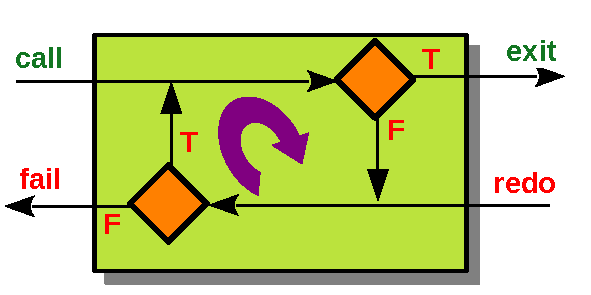
\includegraphics[width=0.90\textwidth, height=0.6\textheight]{figures/trace02.pdf}
\caption{Levemente diferente do que é encontrado na bibliografia!}
\end{center}
\end{figure}

\end{frame}


\begin{frame}[fragile]

\frametitle{Depuração -- uma regra composta}

\begin{figure}[!htb]
\begin{center}
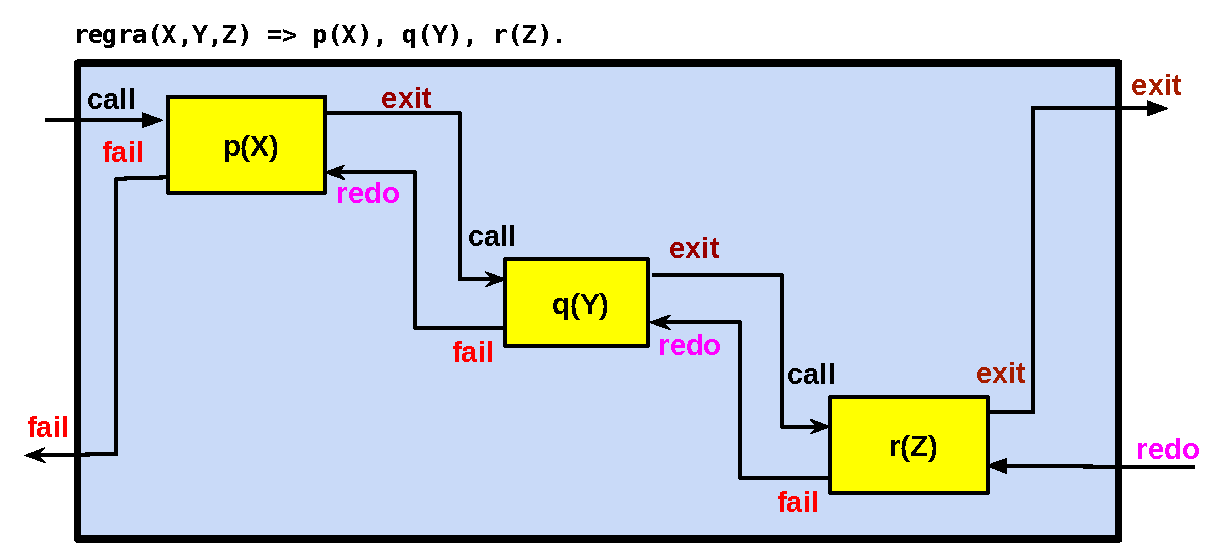
\includegraphics[width=0.90\textwidth, height=0.6\textheight]{figures/trace03.pdf}
%\caption{Realizar buscas com regiões reduzidas -- promissoras (regiões factíveis de soluções)}
\end{center}
\end{figure}

\end{frame}


%%%%%%%%%%%%%%%%%%%%%%%%%%%%%%%%%%%%%%%%%%%%%%%%%%%%
\begin{frame}[fragile]

    \frametitle{Depuração}

    \begin{itemize}
    
      \item Picat tem \textbf{3 modos de execução}: \textit{trace},
      \textit{non-trace} e \textit{spy}
      \pause
      \item  \textit{non-trace}: é a execução normal ou \textit{default} -- vista até o momento

      \pause
      \item  \textit{trace} ou \textit{debug}: vê passo-a-passo de cada variável, predicado ou      função,  do código inteiro
%      \pause
%      \item Uso para fins diversos
      \pause
      \item \textit{spy}: especifica um predicado ou função -- útil para habilitar e desabilitar   partes do código.

      \pause
      \item Devem ser habilitado e desabilitados no \underline{\textbf{modo interpretado}}
    
      \item \textcolor{red}{Há funções e predicados que não tem \textit{backtracking}.}\\
      \pause
       Exemplos: \texttt{nl}, \texttt{printf}, \texttt{read}, etc
       
    \end{itemize}
\end{frame}
%%%%%%%%%%%%%%%%%%%%%%%%%%%%%%%%%%%%%%%%%%%%%%%%%%%%


\begin{frame}[fragile]

\frametitle{Uso básico do \textit{trace}}

\begin{enumerate}
  \item Entre no interpretador do Picat
  
    \item Ative o modo \textit{trace} (ou \textit{debug}), com o comando: \textit{trace}
    
    \item Compile e carregue o programa desejado 
    a depurar, com o comando: \texttt{cl(`....').}
    
    \item Execute a parte desejada do código
    
    \item Vá dando \texttt{Enter} no modo \textit{passo-a-passo}
    
    \item Digite `\textbf{h}' para o \texttt{help}\texttt{\texttt{}}  e ver opções disponíveis
    \item Digite `\textbf{a}' para o \texttt{abortar}\texttt{} o modo trace
      
\end{enumerate}

\end{frame}






%%%%%%%%%%%%%%%%%%%%%%%%%%

\subsection{Trace}
\begin{frame}[fragile]

\frametitle{Exemplo}

\begin{footnotesize}
\begin{verbatim}
index(-)      
     p(2).     p(1).     p(0).
index(-)      
     q(20).    q(22).
%%%%%%%%%%%%%%%%%%%%%%%%%%%%%%%%%%%%%%%%%%%%%% 
regra(X,Y, R) =>   
      p(X),
      q(Y),
      R = X + Y.
%%%%%%%%%%%%%%%%%%%%%%%%%%%%%%%%%%%%%%%%%%%%%% 
main ?=> 
    X + Y = 22
    regra(X,Y, 22) , 
    printf("\n X: %w Y: %w ", X, Y)  ,  
    false.
main =>  printf("\n Não há mais soluções! \n"). 
\end{verbatim}
\end{footnotesize}
\end{frame}


\begin{frame}[fragile]

\frametitle{Considerações de Uso do \textit{trace}}

\begin{itemize}
  \item Este comando é muito útil e se encontra em modo bem
  primitivo de uso
  
  \item Mas, tem \textbf{TUDO} que se precisa para descobrir um erro
  
  \pause
  \item A idéia de se programar com Picat e outras linguagens
  declarativas é: 

  \pause
  \textcolor{magenta}{\textbf{a cada linha de código escrita segue-se por um teste isolado!}}

  \pause
  \item Ou seja,  use o \textit{trace} em partes do código!

  \pause
  \item Ao se ganhar confiança com a linguagem, voce vai omitindo alguns pontos!

  
\end{itemize}

\end{frame}


\begin{frame}[fragile]
\frametitle{Reflexões}

\begin{itemize}
  \item \textcolor{magenta}{Se aprende os detalhes da linguagem com um \textit{trace}}
  
  \pause
    \item Não se assuste com modo \texttt{trace} na console
  
  
  \pause
    \item Atenção na sequência de uso: 
    
    \begin{enumerate}
      \item Ative o modo \textit{trace}
      \item Compile e carregue o seu fonte no modo trace, com o comando \texttt{cl(`.....')}.
      \item Execute o que desejares do código

    \end{enumerate}
    \pause
    Em caso de mudança no código, repita os 3 passos acima
    
\pause
    \item Finalmente, \textit{boas depurações}!        
  
\end{itemize}


\end{frame}
